\documentclass[tikz,border=10pt]{standalone}
\usepackage{tikz}
\begin{document}

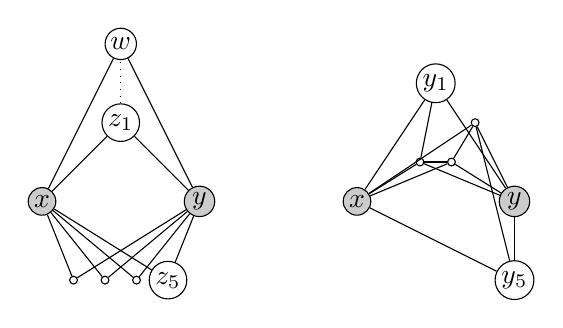
\begin{tikzpicture}[scale=1]
    % Left diagram
    \node[draw, circle, fill=black!20, inner sep=1pt] (x) at (0,0) {$x$};
    \node[draw, circle, fill=black!20, inner sep=1pt] (y) at (2,0) {$y$};
    \node[draw, circle, inner sep=1pt] (w) at (1,2) {$w$};
    \node[draw, circle, inner sep=1pt] (z1) at (1,1) {$z_1$};
    \node[draw, circle, inner sep=1pt] (z2) at (0.4,-1) {};
    \node[draw, circle, inner sep=1pt] (z3) at (0.8,-1) {};
    \node[draw, circle, inner sep=1pt] (z4) at (1.2,-1) {};
    \node[draw, circle, inner sep=1pt] (z5) at (1.6,-1) {$z_5$};

    \draw (x) -- (w);
    \draw (y) -- (w);
    \draw[dotted] (z1) -- (w);
    \draw (x) -- (z1);
    \draw (y) -- (z1);

    \draw (x) -- (z2);
    \draw (x) -- (z3);
    \draw (x) -- (z4);
    \draw (x) -- (z5);

    \draw (y) -- (z2);
    \draw (y) -- (z3);
    \draw (y) -- (z4);
    \draw (y) -- (z5);

    % Right diagram
    \node[draw, circle, fill=black!20, inner sep=1pt] (x2) at (4,0) {$x$};
    \node[draw, circle, fill=black!20, inner sep=1pt] (y2) at (6,0) {$y$};
    \node[draw, circle, inner sep=1pt] (y1) at (5,1.5) {$y_1$};
    \node[draw, circle, inner sep=1pt] (y2a) at (4.8,0.5) {};
    \node[draw, circle, inner sep=1pt] (y3) at (5.2,0.5) {};
    \node[draw, circle, inner sep=1pt] (y4) at (5.5,1) {};
    \node[draw, circle, inner sep=1pt] (y5) at (6,-1) {$y_5$};

    \draw (x2) -- (y1);
    \draw (x2) -- (y2a);
    \draw (x2) -- (y3);
    \draw (x2) -- (y4);
    \draw (x2) -- (y5);

    \draw (y2) -- (y1);
    \draw (y2) -- (y2a);
    \draw (y2) -- (y3);
    \draw (y2) -- (y4);
    \draw (y2) -- (y5);

    \draw (y1) -- (y2a);
    \draw (y2a) -- (y3);
    \draw (y3) -- (y4);
    \draw (y4) -- (y5);
\end{tikzpicture}

\end{document}